\documentclass{article}
\usepackage{graphicx} % Required for inserting images
\usepackage{tabularx}
\usepackage{amssymb}
\usepackage{amsmath}
\usepackage{amsthm}
\usepackage{listings}
\usepackage[swedish]{babel}
\usepackage{hyperref} 
\usepackage{mathtools}
\usepackage{color}
\usepackage{titlesec}
\usepackage{sectsty}
\usepackage[a4paper, margin=2cm]{geometry}
\usepackage{booktabs}
\usepackage{caption}
\usepackage{subcaption}
\usepackage{float}
\usepackage{tikz}


\renewcommand{\thesection}{\arabic{section}.}
\renewcommand{\thesubsection}{\alph{subsection})}
\subsectionfont{\normalfont\bfseries\fontsize{10}{12}\selectfont}

\newcommand{\independent}{\perp\!\!\!\!\perp}

\title{SF1930 Projekt}
\author{Vilhelm Karlin}
\date{\today}

\begin{document}
\maketitle

\section{Uppvärmning}
\subsection{Alla betyg i dataramen är för närvarande tal mellan 0 och 10. 
Normalisera dessa värden i dataramen så att de är mellan 0 och 1.}

För att normalisera datan så itererade jag helt enkelt över de relevanta kolumnerna och dividerade varje värde med 10. 

\subsection{Gör ett histogram för alla trickbetyg för trick 1-4. Vad observerar du? 
Finns det ett visst värde som dyker upp oftare än de andra? Om så är fallet, hur står detta värde i jämförelse med de andra?}

Som syns i figur Fig\ref{fig:1b} så är det enskilt vanligaste värdet 0. Resterande värden är ungefär grupperande mellan 0.7 och 0.9.
Inga värden finns mellan 0.1 och 0.4.

\subsection{For varje trick 1-4 skapa en ny kolumn med namnet 'make i' för i = 1, 2, 3, 4 så att värdet av 'make i' i en given rad är 1 om skateboardåkaren landade trick i och 0 annars.}
Detta implementeras enkelt genom att introducera fyra nya kolumner, en för varje trick. Dessa fylls sedan med 1 om skateboardåkaren landade trick i och 0 annars.

\subsection{För varje skateboardåkare skatta sannolikheten att ett trick får ett betyg som är större än 0.6 givet att 
skateboardåkaren landar tricket. Vad är sannolikheten att skateboardåkaren inte lyckas landa ett visst trick? Vad observerar du? 
Relatera dina observationer till era observationer i del (b).}

Som syns i Tab\ref{tab:1d} så är det endast två skateboardåkare som inte fick betyg större än 0.6 på något av sina gjorda trick.
Detta rimmar väl med observationerna i Fig\ref{fig:1b} där värdena antingen var 0 eller större än runt 0.6.

\subsection{Gör ett spridningsdiagram för runbetyg 1 mot runbetyg 2. Ser du någon tydligt korrelation från diagrammet?} \label{sec:1e}

Korrelationen mellan runbetyg 1 och runbetyg 2 är väldigt svag och ingen tydlig trend kan urskiljas i Fig\ref{fig:1e}.
Korrelationskoefficienten $\rho = 0.19$. Jag anser därmed att det är rimligt att anta att runbetyg 1 och runbetyg 2 är oberoende.

\clearpage  % Start a new page for figures and tables

\begin{figure}[H]
    \centering
    
    \begin{minipage}{0.45\textwidth}
        \centering
        \includegraphics[width=\textwidth]{Figures/1b.png}
        \caption{Histogram för trickbetyg 1-4.}
        \label{fig:1b}
    \end{minipage}
    \hfill
    \begin{minipage}{0.45\textwidth}
        \centering
        \includegraphics[width=\textwidth]{Figures/1e.png}
        \caption{Caption for figure 2.}
        \label{fig:1e}
    \end{minipage}
    
\end{figure}

\begin{table}[H]
    \centering
    \begin{tabular}{lrr}
      \toprule
      $i$ & \textbf{Andel lyckade med betyg större än 0.6} & \textbf{Andel misslyckade trick} \\
      \midrule
      Berger    & 1.00 & 0.83 \\
      Decenzo   & 1.00 & 0.56 \\
      Eaton     & 1.00 & 0.38 \\
      Foy       & 1.00 & 0.50 \\
      Fynn      & 1.00 & 0.50 \\
      Gustavo   & 1.00 & 0.60 \\
      Hoban     & 1.00 & 0.60 \\
      Hoefler   & 1.00 & 0.56 \\
      Horigome  & 1.00 & 0.44 \\
      Huston    & 1.00 & 0.62 \\
      Jordan    & 1.00 & 0.60 \\
      Joslin    & 1.00 & 0.55 \\
      Majerus   & 0.33 & 0.62 \\
      McClung   & 0.00 & 0.75 \\
      Midler    & 1.00 & 0.67 \\
      Milou     & 1.00 & 0.55 \\
      Mota      & 1.00 & 0.75 \\
      Oliveira  & 1.00 & 0.58 \\
      O’neill   & 1.00 & 0.75 \\
      Papa      & 1.00 & 0.56 \\
      Pudwill   & 0.33 & 0.75 \\
      Ribeiro C & 1.00 & 0.75 \\
      Ribeiro G & 1.00 & 0.46 \\
      Rodriguez & 1.00 & 0.50 \\
      Santiago  & 0.00 & 0.92 \\
      Shirai    & 1.00 & 0.60 \\
      Silvas    & 1.00 & 0.62 \\
      Suciu     & 1.00 & 0.38 \\
      Wair      & 1.00 & 0.50 \\
      Wright    & 1.00 & 0.75 \\
      \bottomrule
    \end{tabular}
    \caption{Betyg större än 0.6 givet att skateboardåkaren landar tricket och andel misslyckade trick.}
    \label{tab:1d}
\end{table}
\newpage

\section{En frekventistisk modell.}
\subsection{Ge en punktskattning för varje $\theta_i$, sannolikheten att skateboardåkaren i landar ett trick.}
Via momentmetoden kan vi enklet visa att $\hat{\theta_i} = \frac{1}{n}\sum_{j=1}^n v_{ij}$ är en punktskattning för $\theta_i$ om vi antar att $V_i \sim \text{Ber}(\theta_i)$.
Eftersom $V_i \independent Z_i$ så kan vi helt enkelt tillämpa detta på värdena i 'make i' kolumnerna och får därmed punktskattningarna för $\theta_i$ som visas i Tab\ref{tab:freq_params}. 
\\ \\
Notera att vi endast kommer betrakta skateboardåkare som tävlar i LCQ:n från och med nu.

% Ge en punktskattning för parametrarna [αi,βi]T för varje skateboardåkare i. Finns det skateboardåkare för vilka din valda punktskattning inte existera? I så fall föreslå en alternativ punktskattning för dessa αi, βi. Motivera dina val punktskattningar.
\subsection{Ge en punkskattning för parametrarna $[\alpha_i, \beta_i]^T$ för varje skateboardåkare $i$. 
Finns det skateboardåkare för vilka din valda punktskattning inte existera? 
I så fall föreslå en alternativ punktskattning för dessa $\alpha_i, \beta_i$. Motivera dina val punktskattningar.}

Vi använder momentmetoden för att skatta $\alpha_i$ och $\beta_i$ med hjälp av utfall från $Z_i \sim \text{Beta}(\alpha_i, \beta_i)$.

\begin{equation*}
    \text{E}[Z_i] = \frac{\alpha_i}{\alpha_i + \beta_i}, \text{Var}[Z_i] = \frac{\alpha_i\beta_i}{(\alpha_i + \beta_i)^2(\alpha_i + \beta_i + 1)} \\
\end{equation*}
Vi vill behöver alltså lösa följande system för $\alpha, \beta$ för att få momentmetodens skattningar.
\begin{equation*}
    \bar{z_i} = \frac{\alpha_i}{\alpha_i + \beta_i}, s_i^2 = \frac{\alpha_i\beta_i}{(\alpha_i + \beta_i)^2(\alpha_i + \beta_i + 1)} \\
\end{equation*}
Där $\bar{z_i}$ och $s_i^2$ är stickprovsmedelvärdet och stickprovsvariansen för $Z_i$. Genom att lösa ut $\alpha_i$ och $\beta_i$ ur ekvationerna ovan får vi följande skattningar.

\begin{align}
    \hat{\alpha_i} &= \bar{z_i} (\frac{\bar{z_i}(1-\bar{z_i})}{s_i^2} - 1) \\
    \hat{\beta_i} &= (1-\bar{z_i}) (\frac{\bar{z_i}(1-\bar{z_i})}{s_i^2} - 1)
\end{align}
Skattningarna existerar för alla skateboardåkare förutom Santiago som endast har ett godkänt trick. Han får skattningen $\hat{\alpha}_{\text{Santiago}} = 10 \bar{z}_{\text{Santiago}}, \hat{\beta}_{\text{Santiago}} = 10(1-\bar{z}_{\text{Santiago}})$.
Denna är väntevärdesriktig och ganska konservativ då han har i särklass lägst $E[Z_i]$ av alla skateboardåkare. Samtidigt kommer det ej vara relevant då $\hat{\theta}_{\text{Santiago}} = 0.08$ är så låg att han ej kommer kunna kvalificera sig till finalen.
Punkskattningarna kan ses i Tab\ref{tab:freq_params}.

\subsection{Föreslå en modell för $Y_i$ och ge en punktskattning för dina modells parametrar. Motivera dina val för modell och punktskattning.}
Utifrån observationen från del 1\ref{sec:1e} så antar vi att $Y_{i1}, Y_{i2}$ är oberoende och likafördelade.
Vi kan därmed även modellera runs med en betafördelning, nämligen $Y_i \sim \text{Beta}(a_i, b_i)$. 
Vi tillämpar momentmetoden för att skatta $a_i, b_i$, precis som ovan och resultatet kan ses i Tab\ref{tab:freq_params}.

\subsection{Använd din modell för $[X_i,Y_i]^T$ för att simulera 5000 LCQ:ar och för varje simulering extrahera de fyra skateboardåkare $\vec{W} = [W_1,W_2,W_3,W_4]^T$ med
de högsta totalbetygen. Vad är typvärdet för $\vec{W}_1, ..., \vec{W}_{5000}$? De riktiga vinnarna för LCQ:en är Gustavo, Hoban, Eaton, Decenzo.
Hur många av de riktiga vinnarna förutsägs av typvärdet? Vad är skattade sannolikheten för de riktiga vinnarna baserat på dina simuleringar? Av typvärdet?}

För att simulera en skateboardåkares totala poäng under ett LCQ så kan vi helt enkelt använda våra punkskattningar för att
simulera 4 $X_i$ och 2 $Y_i$, sedan kan vi summera den största $Y_i$ och de två största $X_i$ för att få totalpoängen för den tävlingen.
Vi kör sedan 5000 sådana simuleringar för varje skateboardåkare och därmed får vi våra 5000 $\mathbf{W}_j$.
\\ \\
Typvärdet är Eaton, Hoban, Jordan, Shirai. Denna sker i 1.08\% av fallen. Sannolikheten för de riktiga vinnarna är 0.04\%. 
Om vi betraktar utfallen individuellt får vi att de vanligaste top 4 medlemmarna är Eaton (49\%), Jordan (48\%), Shirai (46\%) och Hoban (43\%). 
Gustavo och Decenzo har sannolikheterna 31\% och 33\% att vara top 4.

\begin{table}[t]
    \centering
    \caption{Frequentistiska punktskattningar för skateboardåkarna.}
    \label{tab:freq_params}
    \begin{tabular}{lrrrrr}
        \toprule
        i & $\hat{\theta}$ & $\hat{\alpha}$ & $\hat{\beta}$ & $\hat{a}$ & $\hat{b}$ \\
        \midrule
        Decenzo   & 0.44 & 24.46 & 5.11 & 4.16 & 2.83 \\
        Eaton     & 0.62 & 75.41 & 20.05 & 103.57 & 36.87 \\
        Foy       & 0.50 & 51.59 & 9.10 & 3.51 & 4.09 \\
        Gustavo   & 0.40 & 70.64 & 17.52 & 1.23 & 0.86 \\
        Hoban     & 0.40 & 107.70 & 15.03 & 3.63 & 2.10 \\
        Hoefler   & 0.44 & 32.52 & 9.40 & 1.75 & 0.97 \\
        Jordan    & 0.40 & 23.06 & 3.64 & 3.61 & 1.23 \\
        Majerus   & 0.38 & 2.91 & 2.72 & 1.76 & 2.47 \\
        Midler    & 0.33 & 43.72 & 10.42 & 1.29 & 0.82 \\
        Mota      & 0.25 & 24.01 & 6.77 & 4.06 & 4.57 \\
        Oliveira  & 0.42 & 68.88 & 17.87 & 5.39 & 4.04 \\
        O'neill   & 0.25 & 1252.67 & 232.71 & 0.60 & 0.73 \\
        Papa      & 0.44 & 22.31 & 6.35 & 2.16 & 2.07 \\
        Ribeiro C & 0.25 & 194.78 & 56.01 & 1.80 & 1.52 \\
        Santiago  & 0.08 & 4.70 & 5.30 & 2.68 & 4.34 \\
        Shirai    & 0.40 & 20.58 & 2.35 & 1.84 & 1.10 \\
        \bottomrule
    \end{tabular}
\end{table}

\newpage
\section{En bayesiansk modell.}

\subsection{Föreslå en simultan apriorifördelning för parametrarna $[\theta_i, \alpha_i, \beta_i]^T$ för $X_i$ där vi antar $\theta_i \independent \alpha_i, \beta_i$ för alla $i$. Motivera ditt val.}

$\Theta_i \independent A_i, B_i \implies f_{\Theta_i, A_i, B_i}(\theta_i, \beta_i, \alpha_i)=f_{\Theta_i}(\theta_i) f_{A_i, B_i}(\alpha_i, \beta_i)$,
och vi kan därmed behandla $\Theta_i$ och $A_i, B_i$ separat. 

$V_i | \Theta_i = \theta_i \sim Ber(\theta_i)$ har som konjugerad apriorifördelning $Beta(c_i, d_i)$, och vi kommer därmed använda den.
$Z_i | A_i = \alpha_i, B_i = \beta_i \sim Beta(\alpha_i, \beta_i)$ har ingen konjugerad apriorifördelning och är därmed ganska knepig.
Exempel 10.8 från föreläsningarna erbjuder ett bra förslag för en apriorifördelning för $\alpha_i, \beta_i$.
Den bygger på en omparameterisering till dess väntevärde och precisionsmått, $\mu_i = \frac{\alpha_i}{\alpha_i + \beta_i}, \kappa_i = \alpha_i + \beta_i + 1$.
Vi kan då bilda en apriorifördelning, $f_{\mu_i, \kappa_i}(\mu_i, \kappa_i) = f_{\kappa_i | \mu_i}(\kappa_i | \mu_i) f_{\mu_i}(\mu_i)$, där $\kappa_i | \mu_i \sim Gamma(\phi_i, \lambda_i)$ och $\mu_i \sim U(0,1)$.
Detta ger oss fördelningen:
\[
    f_{A_i, B_i}(\alpha_i, \beta_i) = \frac{\lambda^{\phi_i}}{\Gamma(\phi_i)} (\alpha_i + \beta_i + 1)^{\phi_i - 1} e^{-\lambda_i(\alpha_i + \beta_i + 1)} (\alpha_i + \beta_i)^{-1}  
\]
Sammansatt får vi följande funktion för den simultana apriorifördelningen:
\[ 
    f_{\Theta_i, A_i, B_i}(\theta_i, \alpha_i, \beta_i) = 
    (\frac{\Gamma(c_i + d_i)}{\Gamma(c_i) \Gamma(d_i)} \theta_i^{c_i-1} (1-\theta_i)^{d_i-1}) 
    (\frac{\lambda^{\phi_i}}{\Gamma(\phi_i)} (\alpha_i + \beta_i + 1)^{\phi_i - 1} e^{-\lambda_i(\alpha_i + \beta_i + 1)} (\alpha_i + \beta_i)^{-1}) 
\]

\subsection{Generera 5000 slumpmässiga utfall från aposteriorifördelningarna $f_{\Theta_i, A_i, B_i | X_i}(\theta_i, \alpha_i, \beta_i | x_i)$.
Plotta dina resulterande utfall för de marginella aposteriorifördelningarna: \\
$f_{\Theta_i | X_i}(\theta_i | x_i)$ och $f_{A_i, B_i | X_i}(\alpha_i, \beta_i | x_i)$. \\
Beräkna det aposteriori stickprovsmedelvärdet och den aposteriori stickprovvariansen för varje parameter $\theta_i, \alpha_i, \beta_i$ för alla skateboardåkare.}

Jag använder mig av Metropolisalgoritmen för att generera 5000 slumpmässiga utfall från aposteriorifördelningarna.
Metropolisalgoritmen har dessutom har den trevliga egenskapen att jag inte behöver kunna normalisera fördelningen.
Jag använder därmed följande:
\begin{align*}
    f_{\Theta_i, A_i, B_i | \mathbf{X}}(\theta_i, \alpha_i, \beta_i | \mathbf{x}) &\propto f_{\mathbf{X} | \Theta_i, A_i, B_i}(\mathbf{x} | \theta_i, \alpha_i, \beta_i) f_{\Theta_i, A_i, B_i}(\theta_i, \alpha_i, \beta_i) \\
    &\propto \theta_i^{c_i-1} (1-\theta_i)^{d_i-1} (\alpha_i + \beta_i + 1)^{\phi_i - 1} e^{-\lambda_i(\alpha_i + \beta_i + 1)} (\alpha_i + \beta_i)^{-1} \prod\limits_{j=1}^4 f_{X_j | \Theta_i, A_i, B_i}(x_j | \theta_i, \alpha_i, \beta_i)
\end{align*}
Till Metropolisalgoritmen använde jag en standardiserad normalfördelning med standardavvikelse, $\sigma = 0.5$ som hoppfördelning,
4 kedjor, 6000 iterationer per kedja (1000 burn-in iterationer) där jag använde punktskattningarna från ovan som startvärden.
För att få olika startvärden för varje kedja så adderade jag till varje startvärde med $e^q$, där $q$ kommer från en Cauchyfördelning med skalfaktor 0.05.
\\\\
Efter lite experementation fann jag parametrar till apriorifördelningen som gav rimliga resultat. 
Jag använde $c_i=d_i=1$, som val för en icke-informativ fördelning för $\Theta_i$. För $A_i, B_i$, använde jag $\lambda_i=0.5, \phi_i=5$.
Resultaten från min simulering, efter burn-in, kan ses i Fig\ref{fig:3b} och Tab\ref{tab:bayes_params}.

% Föreslå en (simultan) apriorifördelning för parametrarna för din modell Yi från uppgift 2(c) och motivera ditt val. Du får anta att modellens parame- trar för skateboardåkaren i är oberoende av alla andra parametrar inklusive θi,αi och βi. Generera 5000 utfall från aposteriorifördelningen (se till att spara dessa utfall!) och gör ett spridningsdiagram av resultatet. Vad är stick- provsmedelvärdet och stickprovsvariansen för var och en av dina parametrar baserat på dina utfall?
\subsection{Föreslå en (simultan) apriorifördelning för parametrarna för din modell $Y_i$ från uppgift 2(c) och motivera ditt val.
Du får anta att modellens parametrar för skateboardåkaren $i$ är oberoende av alla andra parametrar inklusive $\theta_i, \alpha_i$ och $\beta_i$. 
Generera 5000 utfall från aposteriorifördelningen (se till att spara dessa utfall!) och gör ett spridningsdiagram av resultatet.
Vad är stickprovsmedelvärdet och stickprovsvariansen för var och en av dina parametrar baserat på dina utfall?}

Likt i den frequentistiska modellen så antar vi att $Y_i | \mathcal{A}_i = a_i, \mathcal{B}_i = b_i \sim Beta(a_i, b_i)$. 
Vi kan då använda samma apriorifördelning för $\mathcal{A}_i, \mathcal{B}_i$ som användes för $A_i, B_i$ för $X_i$. Vi använder samma $\lambda_i, \phi_i$ som för $A_i, B_i$ och vi använder Metropolisalgoritmen med samma kedjor, hoppfördelning och knep för startvärdena som ovan och aposteriorifördelningen:
\begin{align*}
    f_{\mathcal{A}_i, \mathcal{B}_i | \mathbf{Y}}(a_i, b_i | \mathbf{y}) &\propto f_{\mathbf{Y} | \mathcal{A}_i, \mathcal{B}_i}(\mathbf{y} | a_i, b_i) f_{\mathcal{A}_i, \mathcal{B}_i}(a_i, b_i) \\
    &\propto (a_i + b_i + 1)^{\phi_i - 1} e^{-\lambda_i(a_i + b_i + 1)} (a_i + b_i)^{-1} \prod\limits_{j=1}^2 f_{Y_j | \mathcal{A}_i, \mathcal{B}_i}(y_j | a_i, b_i)
\end{align*}
Plottarna för de aposteriora fördelningarna kan ses i Fig\ref{fig:3c} och dess nyckeltal i Tab\ref{tab:bayes_params}.

\subsection{Använd din bayesiansk modell för $[X_i,Y_i]^T$ för att simulera 5000 LCQ:ar genom att ta utfall från de lämpliga de aposteriori prediktiva fördelningarna.
Vad är typvärdet av dina utfall $W_1,...,W_{5000}$? Hur många av de riktiga vinnarna förutsägs? Vad är den skattade sannolikheten för de riktiga vinnarna baserat på dina utfall? Av typvärdet?}

Samma metod som för den frekventistiska modellen användes för att simulera LCQ:ar. 
Den enda skillnaden är att olika värden för parametrarna användes för varje LCQ, där jag slumpade fram 1250 stickprov från varje kedja.
\\\\
Typvärdet är Eaton, Hoban, Jordan, Shirai. Denna sker i 1.5\% av fallen. Sannolikheten för de riktiga vinnarna är 0.052\%. 
Om vi betraktar utfallen individuellt får vi att de vanligaste top 4 medlemmarna är Eaton (55\%), Jordan (45\%), Shirai (42\%) och Hoban (42\%). 
Gustavo och Decenzo har sannolikheterna 30\% och 35\% att vara top 4.

\begin{table}[H]
    \centering
    \caption{Aposteriori stickprovsmedelvärdet och den aposteriori stickprovsorvariansen för $\theta_i, \alpha_i, \beta_i$}
    \label{tab:bayes_params}
    \begin{tabular}{l|rr|rr|rr|rr|rr}
        \toprule
        i & $\bar{\theta}$ & $s_{\theta}^2$ & $\bar{\alpha}$ & $s_{\alpha}^2$ & $\bar{\beta}$ & $s_{\beta}^2$ & $\bar{a}$ & $s_{a}^2$ & $\bar{b}$ & $s_{b}^2$ \\
        \midrule
        Decenzo & 0.41 & 0.01 & 14.03 & 19.73 & 3.05 & 1.03 & 6.02 & 3.77 & 3.96 & 1.68 \\
        Eaton & 0.55 & 0.02 & 14.06 & 22.63 & 3.97 & 2.04 & 12.79 & 19.26 & 4.81 & 3.15 \\
        Foy & 0.46 & 0.02 & 15.56 & 24.17 & 2.97 & 1.04 & 4.29 & 2.35 & 5.42 & 3.56 \\
        Gustavo & 0.38 & 0.01 & 16.15 & 24.38 & 4.24 & 1.72 & 2.56 & 0.74 & 1.84 & 0.36 \\
        Hoban & 0.38 & 0.01 & 18.08 & 32.30 & 2.83 & 0.84 & 5.41 & 2.94 & 3.00 & 0.89 \\
        Hoefler & 0.42 & 0.01 & 13.78 & 19.61 & 4.14 & 1.94 & 2.56 & 0.84 & 1.73 & 0.39 \\
        Jordan & 0.38 & 0.01 & 15.91 & 24.94 & 2.70 & 0.77 & 6.74 & 4.45 & 2.29 & 0.51 \\
        Majerus & 0.34 & 0.02 & 5.76 & 5.20 & 5.24 & 4.24 & 3.28 & 1.83 & 5.17 & 4.17 \\
        Midler & 0.31 & 0.02 & 13.33 & 23.08 & 3.37 & 1.83 & 1.60 & 0.45 & 1.51 & 0.41 \\
        Mota & 0.22 & 0.01 & 11.61 & 18.87 & 3.38 & 2.09 & 5.54 & 3.45 & 6.05 & 4.18 \\
        Oliveira & 0.38 & 0.02 & 14.10 & 24.66 & 3.93 & 2.21 & 6.86 & 5.46 & 4.95 & 2.96 \\
        O’neill & 0.24 & 0.01 & 14.20 & 27.12 & 2.95 & 1.69 & 1.73 & 0.47 & 2.25 & 0.77 \\
        Papa & 0.40 & 0.01 & 13.04 & 17.59 & 3.80 & 1.59 & 3.74 & 1.64 & 3.67 & 1.51 \\
        Ribeiro C & 0.24 & 0.01 & 12.94 & 20.33 & 3.96 & 2.59 & 3.69 & 1.88 & 3.28 & 1.47 \\
        Santiago & 0.07 & 0.00 & 6.86 & 10.75 & 7.73 & 12.53 & 3.93 & 1.89 & 6.64 & 5.13 \\
        Shirai & 0.38 & 0.01 & 15.63 & 23.94 & 1.93 & 0.40 & 2.57 & 0.74 & 1.68 & 0.30 \\
        \bottomrule
    \end{tabular}
\end{table}

\begin{figure}[htbp]
    \centering
    \includegraphics[width=1\textwidth]{Figures/3b.png}
    \caption{Aposterori fördelningar för $\theta_i, \alpha_i, \beta_i$}
    \label{fig:3b}
\end{figure}


\begin{figure}[t]
    \centering
    \includegraphics[width=1\textwidth]{Figures/3c.png}
    \caption{Aposterori fördelningar för $a_i, b_i$}
    \label{fig:3c}
\end{figure}

\subsection{I modellen i uppgift 3(d) antog vi att parametrarna $Y_i$ för $Y_i$ och parametrarna $\Theta_i = [\Theta_i, A_i, B_i]^T$ för $X_i$ är oberoende givet data (varför?).
Samtidigt antog vi inte att $\Theta_i \independent A_i, B_i$ är oberoende givet data.
Låt $X_i^{(1)}, X_i^{(2)}, X_i^{(3)}, X_i^{(4)}$ betecknar skateboardåkare $i$:s fyra trickbetyg, låt $Y_i^{(1)}, Y_i^{(2)}$ betecknar skateboardåkare $i$:s två runbetyg och låt $O_i$ betecknar deras totalbetyg.
Rita en acyklisk riktad graf med så få kanter som möjligt så att den simultana fördelningen för $O_i, X_i^{(1)}, X_i^{(2)}, X_i^{(3)}, X_i^{(4)}, Y_i^{(1)}, Y_i^{(2)}, \Theta_i, A_i, B_i$ och $Y_i$ är markovsk med avseende på den.
med avseende på den. Baserat på din graf kan du dra slutsatsen att den marginella aposteriorifördelningen för $\Theta_i, A_i, B_i$ faktoriserar som 
\\$f_{\Theta_i, A_i, B_i | X_i}(\theta_i, \alpha_i, \beta_i | x_i) = f_{\Theta_i | X_i}(\theta_i | x_i)f_{A_i, B_i | X_i}(\alpha_i, \beta_i | x_i)$?
Betrakta dina parametrarna $\Theta_i$ för $Y_i$ och parametrarna $\Theta_i$ för $X_i$. \\Enligt din graf är vårt antagande att $\Theta_i \independent \Theta_i | X_i^{(1)}, X_i^{(2)}, X_i^{(3)}, X_i^{(4)}, Y_i^{(1)}, Y_i^{(2)}$ vettigt?
Kan vi anta oberoenderelationen $\Theta_i \independent \Theta_i | O_i$ om bara datan $o_i$ är givet istället?}

\begin{figure}[h]
    \centering
    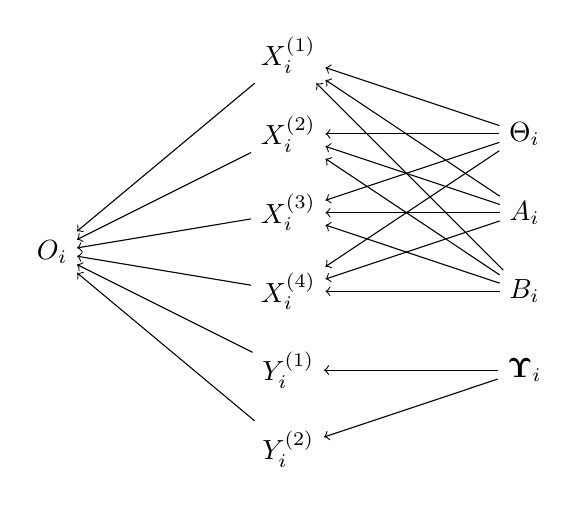
\begin{tikzpicture}
        \centering
        % Nodes
        \node (theta) at (6, 4) {$\Theta_i$};
        \node (a) at (6, 3) {$A_i$};
        \node (b) at (6, 2) {$B_i$};
        \node (upsilon) at (6, 1) {$\mathbf{\Upsilon}_i$};
        \node (x1) at (3, 5) {$X_i^{(1)}$};
        \node (x2) at (3, 4) {$X_i^{(2)}$};
        \node (x3) at (3, 3) {$X_i^{(3)}$};
        \node (x4) at (3, 2) {$X_i^{(4)}$};
        \node (y1) at (3, 1) {$Y_i^{(1)}$};
        \node (y2) at (3, 0) {$Y_i^{(2)}$};
        \node (o) at (0, 2.5) {$O_i$};
        % Edges
        \draw[->] (theta) -- (x1);
        \draw[->] (theta) -- (x2);
        \draw[->] (theta) -- (x3);
        \draw[->] (theta) -- (x4);
        \draw[->] (a) -- (x1);
        \draw[->] (a) -- (x2);
        \draw[->] (a) -- (x3);
        \draw[->] (a) -- (x4);
        \draw[->] (b) -- (x1);
        \draw[->] (b) -- (x2);
        \draw[->] (b) -- (x3);
        \draw[->] (b) -- (x4);
        \draw[->] (upsilon) -- (y1);
        \draw[->] (upsilon) -- (y2);
        \draw[->] (x1) -- (o);
        \draw[->] (x2) -- (o);
        \draw[->] (x3) -- (o);
        \draw[->] (x4) -- (o);
        \draw[->] (y1) -- (o);
        \draw[->] (y2) -- (o);
    \end{tikzpicture}
    \caption{LCQ graf, $\mathcal{G}$}
    \label{fig:hierarki}
\end{figure}
Vi antog att $\mathbf{\Theta} \independent \mathbf{\Upsilon} | \mathbf{X} = \mathbf{x}$ eftersom trick och runs är olika kategorier i tävlingen och den enas data bör därmed ej påverka den andras fördelning.
Dessutom gör det modellen enklare.
\\\\
Enligt grafen så är det tyligt att $\Theta_i \not\independent A_i, B_i | \mathbf{X}$ då information kan flöda från $\Theta_i$ till $A_i, B_i$ via $\mathbf{X}$ eftersom $\Theta_i, A_i, B_i$ alla är föräldrar till $\mathbf{X}$.
Eftersom våra stokastiska variablar är markovska med avseende på $\mathcal{G}$ så gäller:
\[
    f_{\Theta_i, A_i, B_i | X_i}(\theta_i, \alpha_i, \beta_i | x_i) \neq f_{\Theta_i | X_i}(\theta_i | x_i)f_{A_i, B_i | X_i}(\alpha_i, \beta_i | x_i)
\]
Grafen visar att $\mathbf{\Upsilon} \independent \mathbf{\Theta} | X_i^{(1)}, X_i^{(2)}, X_i^{(3)}, X_i^{(4)}, Y_i^{(1)}, Y_i^{(2)}$, då det inte finns någon stig mellan våra $\mathbf{X}_i$ och $\mathbf{Y}_i$.
Däremot är $\mathbf{\Upsilon} \not\independent \mathbf{\Theta} | O_i$ då båda $\mathbf{\Upsilon}$ och $\mathbf{\Theta}$ är förfädrar till $O_i$.

\newpage
\section{En bayesiansk modell med en hierarki.}

% Anta att Θi|Ci = ci, Di = ci ∼ Beta(ci, di) och välj en lämplig simultan apri- orifördelning för [Θi, Ci, Di]T . (Här är Ci och Di hyperparametrarna för den bayesianska hierarkiska modellen som i råttorna exemplet i föreläsning 11.) Motivera ditt val.
\subsection{Anta att $\Theta_i | C_i = c_i, D_i = d_i \sim Beta(c_i, d_i)$ och välj en lämplig simultan apriorifördelning för $[\Theta_i, C_i, D_i]^T$.
(Här är $C_i$ och $D_i$ hyperparametrarna för den bayesianska hierarkiska modellen som i råttorna exemplet i föreläsning 11.) Motivera ditt val.}

Eftersom varje tävling nu behandlas separat, och det enda värdet vi är intresserade av att undersöka ytterligare är $\Theta_i$,
så kan vi introducera en ny variabel $E_i = \sum\limits_{j=1}^4 V_i^{(j)}$ som representerar antalet godkända trick under en tävling.
Eftersom $X_i^{(j)} \independent X_i^{(k)} | \Theta_i = \theta$ givet $j \neq k$ så har vi att $E_i | \Theta_i = \theta \sim \text{Bin}(4, \theta)$.

Vi kan nu använda oss av samma hierarkiska modell som i råttexemplet från föreläsningarna. Vi utnyttjar att:
\[
    f_{C_i, D_i | \mathbf{E_i}}(c_i, d_i | \mathbf{e_i}) = \frac{f_{\mathbf{\Theta}_i, C_i, D_i | \mathbf{E_i}}(\mathbf{\theta}_i, C_i, D_i | \mathbf{e_i})}{f_{\mathbf{\Theta}_i | C_i, D_i, \mathbf{E_i}}(\mathbf{\theta}_i | C_i, D_i, \mathbf{e_i})}
\]
Den simultana apriorifördelningen blir:
\begin{align*}
    f_{\mathbf{\Theta}_i, C_i, D_i | \mathbf{E_i}}(\theta_i, C_i, D_i | \mathbf{e_i}) &\propto f_{C_i, D_i}(c_i, d_i) f_{\mathbf{\Theta}_i | C_i, D_i}(c_i, d_i) f_{\mathbf{E_i} | \mathbf{\Theta}_i, C_i, D_i}(\mathbf{e_i} | \mathbf{\theta}_i, c_i, d_i) \\
    &\propto f_{C_i, D_i}(c_i, d_i) \prod\limits_{j=1}^m \frac{\Gamma(c_i + d_i)}{\Gamma(c_i) \Gamma(d_i)} \theta_i^{c_i-1} (1-\theta_i)^{d_i-1} \prod\limits_{j=1}^m \binom{4}{e_{i,j}} \theta_i^{e_{i,j}} (1-\theta_i)^{4-e_{i,j}} \\
\end{align*}
Där vi har $m$ olika tävlingar som skateboardåkare $i$ deltar i. Vår uppdateringsregel ger oss att $\Theta_i | E_i = e_i, C_i = c_i, D_i = d_i \sim Beta(c_i + e_i, d_i + 4 - e_i)$.
Alla olika tävlingar, $j = 1, ..., m$ för skateboardåkare $i$ ger oss:
\[
    f_{\mathbf{\Theta}_i | C_i, D_i, \mathbf{E_i}}(\mathbf{\theta} | c_i, d_i, \mathbf{e_i}) = \prod\limits_{j=1}^{m} \frac{\Gamma(c_i + d_i + 4)}{\Gamma(c_i + e_{i,j}) \Gamma(d_i + 4 - e_{i,j})} \theta^{c_i + e_{i,j} - 1} (1-\theta)^{d_i + 4 - e_{i,j} - 1}
\]
Sammansatt får vi följande funktion för den simultana apriorifördelningen för hyperparametrarna $C_i, D_i$.
\[
    f_{C_i, D_i | \mathbf{E_i}}(c_i, d_i | \mathbf{e_i}) \propto f_{C_i, D_i}(c_i, d_i) \prod\limits_{j=1}^m \frac{\Gamma(c_i + d_i)}{\Gamma(c_i) \Gamma(d_i)} \frac{\Gamma(c_i + e_{i,j}) \Gamma(d_i + 4 - e_{i,j})}{\Gamma(c_i + d_i + 4)}
\]
Eftersom $\Theta_i | C_i = c_i, D_i = d_i \sim \text{Beta}(c_i, d_i)$ så kan vi använda samma apriorifördelning för $C_i, D_i$ som tidigare, dvs. den från Exempel 10.8 i föreläsningarna.

\subsection{Generera 5000 slumpmässiga utfall från den simultana aposteriorifördelningen $f_{C_i, D_i | X_i}(c_i, d_i | x_i)$.
Använd dina simuleringar för att generera 5000 slumpmässiga utfall från den marginella aposteriorifördelningen $\Theta_i | X_i = x_i$.
Gör diagram med dina utfall för följande aposteriorifördelningar: $f_{\Theta_i | X_i}(\theta_i | x_i)$ och $f_{C_i, D_i | X_i}(c_i, d_i | x_i)$.
Ge skattningar för aposterioriväntevärdet och aposteriorivariansen för var och en av parametrarna.
Hur jämför dessa varianser för $\theta_i$ med varianserna för $\theta_i$ beräknade för modellen i Uppgift 3?}

Vi använder samma metod med Metropolisalgoritmen som i Uppgift 3 för att generera 5000 slumpmässiga utfall från den simultana aposteriorifördelningen. Den enda skillanden är att vi använder $\sigma = 0.1$ i hoppfördelningen.
Startgissningarna ges än en gång av punkskattningar via momentmetoden. Samma metod användes som tidigare användes för Santiago ifall endast en kedja existerar eller om momentmetoden ger $(0,0)$.
\\\\
Genom att använda dessa 5000 utfall från $C_i, D_i$ från de olika kedjorna kan vi generera 5000 utfall av $\Theta_i$ från en betafördelning med parametrar $c_i, d_i$.
\\\\
Resultaten från min simulering, efter burn-in, kan ses i Fig\ref{fig:4b} och Tab\ref{tab:hierarkisk_params}.
Från tabellen kan man se att variansen i snitt är ungefär dubbelt så stor som i Uppgift 3.
Detta är rimligt i och med att vi nu har hyperparametrar med egen varians istället för punktskattnignar för $C_i, D_i$.

% Med hjälp av dina 5000 utfall från del (b) simulera 5000 LCQ tävlingsvinnare och beräkna typvärdet av resultatet. Vilka är de respektive skattade sanno- likheterna för de riktiga vinnarna och ditt typvärde?
\subsection{Med hjälp av dina 5000 utfall från del (b) simulera 5000 LCQ tävlingsvinnare och beräkna typvärdet av resultatet.
Vilka är de respektive skattade sannolikheterna för de riktiga vinnarna och ditt typvärde?}

Jag använder dessa 5000 utfall av $\Theta_i$ tillsammans med de frekventistiska punktskattningarna för parametrarna i $Z_i, Y_i$ för att simulera LCQ:ar.
\\\\
Typvärdet är Eaton, Hoban, Jordan, Shirai. Denna sker i 1.22\% av fallen. Sannolikheten för de riktiga vinnarna är 0.042\%. 
Om vi betraktar utfallen individuellt får vi att de vanligaste top 4 medlemmarna är Jordan (50\%), Shirai (46\%), Hoban (43\%) och Eaton (42\%). 
Gustavo och Decenzo har sannolikheterna 30\% och 34\% att vara top 4.

\begin{table}[h]
    \centering
    \caption{Aposteriori stickprovsmedelvärdet och den aposteriori stickprovsorvariansen för $\theta_i, c_i, d_i$}
    \label{tab:hierarkisk_params}
    \begin{tabular}{l|rr|rr|rr}
    \toprule
    $i$ & $\bar{\theta}$ & $s_{\theta}^2$ & $\bar{c}$ & $s_{c}^2$ & $\bar{d}$ & $s_{d}^2$ \\
    \midrule
    Decenzo   & 0.44 & 0.03 & 6.75 & 11.82 & 8.44 & 13.70 \\
    Eaton     & 0.60 & 0.05 & 9.29 & 23.63 & 6.08 & 15.88 \\
    Foy       & 0.50 & 0.04 & 7.58 & 13.73 & 7.31 & 12.30 \\
    Gustavo   & 0.39 & 0.03 & 5.81 & 8.09 & 8.82 & 13.79 \\
    Hoban     & 0.41 & 0.03 & 6.54 & 9.77 & 9.49 & 17.52 \\
    Hoefler   & 0.45 & 0.03 & 6.52 & 11.23 & 7.90 & 12.25 \\
    Jordan    & 0.41 & 0.03 & 6.65 & 8.58 & 9.46 & 17.52 \\
    Majerus   & 0.38 & 0.04 & 6.03 & 13.44 & 9.41 & 17.93 \\
    Midler    & 0.32 & 0.03 & 5.03 & 7.64 & 10.38 & 16.93 \\
    Mota      & 0.27 & 0.03 & 3.93 & 5.38 & 11.28 & 20.58 \\
    Oliveira  & 0.43 & 0.04 & 6.93 & 14.17 & 9.23 & 17.13 \\
    O’neill   & 0.26 & 0.03 & 3.83 & 5.996 & 11.08 & 21.86 \\
    Papa      & 0.44 & 0.03 & 6.60 & 8.92 & 8.39 & 12.91 \\
    Ribeiro C & 0.25 & 0.03 & 3.87 & 4.83 & 11.74 & 22.32 \\
    Santiago  & 0.10 & 0.01 & 1.51 & 2.13 & 13.75 & 33.70 \\
    Shirai    & 0.40 & 0.03 & 6.67 & 8.70 & 9.80 & 15.01 \\
    \bottomrule
    \end{tabular}
\end{table}

\begin{figure}
    \centering
    \includegraphics[width=1\textwidth]{Figures/4b.png}
    \caption{Aposterori fördelningar för $\theta_i, c_i, d_i$}
    \label{fig:4b}
\end{figure}

\newpage
\section{Diskussion.}

\subsection{Hur jämför resultaten (skateboardåkarna i typvärdena) av de olika modellerna? Vilka skateboardåkare är korrekt förutspådda och vilka inte är det? Ge några möjliga förklaringar till skillnaderna mellan de olika modellernas förutsägelser. Vilken modell föredrar du och varför?}
Intressant nog så har jag fått exakt samma typvärde för alla modeller. Detta är dock inte helt orimligt med tanke på att alla modeller bygger på samma data.
En intressant skillnad i den hierarkiska modellen är att den tidigare storfavoriten, Eaton, nu 'bara' ligger på fjärde plats som individ.
En rimlig förklaring till detta är att den hierarkiska modellen har en större varians i $\theta_i$ än den andra modellerna.
Som syns i Tab\ref{tab:freq_params} så är Eatons kankse största styrka att han har högst $\theta_i$ av alla skateboardåkare.
Detta håller i alla modeller, men en hypotes skulle vara att den stora variansen i den hierarkiska modellen gör att någon av de många andra åkare lyckas utprestera honom oftare i tävlingarna.
\\\\
Jag föredrar den vanliga Bayesianska modellen då denna använder aposteriorifördelningar för alla parametrar istället för att endast göra detta för $\Theta_i$.
En bayesiansk metod känns mest lämplig eftersom vi har så få tävlingar att dra slutsatser ifrån, vilket gör den frekventistiska metoden mindre lämplig.
En intressant vidareutveckling hade varit att använda en hierarkisk modell för alla parametrar tillsammans med någon slags 'dagsforms'-hyperparameter då jag anser att det finns en viss nytta i att betrakta olika tävlingar separat.

\subsection{Hur jämför dina skattningar för $\theta_i$ i Uppgift 1 och dina skattade väntevärden och varianser för $\theta_i$ i Uppgift 3 och 4? Vad är det förväntade betyget för ett trick för varje skateboardåkare givet att tricket har lyckats landa? Vad är det förväntade runbetyget? Med tanke på skateboardåkare som förutspås vinna enligt de olika modellerna, ger dessa statistikor några insikter om framgångsrika strategier för att vinna? (Till exempel, fungerar det att fokusera på ett bra runbetyg framför bra trickbetyg? Finns det exempel där denna strategi fungerar? Är det bra att ha bättre trickbetyg med stor varians eller lite sämre trickbetyg med mindre varians? osv.)}
Skattningarna för $\theta_i$ i Uppgift 1 och Uppgift 3 är väldigt lika, vilket är rimligt då de använder samma data.
Dock så har modellen i uppgift 4 mycket högre varians än den i Uppgift 3 (och den frekventistiska modellen har 0 varians).
\\\\
Både $Z_i, Y_i$ är betafördelade så vi använder $E[X] = \frac{\alpha}{\alpha + \beta}$ för att beräkna det förväntade betyget för ett lyckat trick eller run.
Resultaten kan ses i Tab\ref{tab:exp_scores}. De som oftast är med i topp fyran för alla våra fördelningar är Jordan, Shirai, Hoban och Eaton.
Nästan alla åkare har högre snittbetyg för ett lyckat trick än för en run och våra vinnare står inte märkvärt ut, bortsätt från Shirai som har betydligt högre väntevärde för lyckade trick än run.
Detta känns dock som en rimlig strategi då två trick räknas in i poängen medans bara en run räknas in. Fler poäng kan alltså samlas från runs.
Att ha högre varians bör också belönas då endast de bästa resultaten räknas för både tricks och runs.
Det som datan visar tydligast däremot är dock att det viktigaste är att ha höga väntevärden för lyckade trick och runs, vilket är rimligt.

\begin{table}[h]
    \centering
    \caption{Väntevärden för lyckade trick, runs och väntevärde och varians för totalbetyg.}
    \label{tab:exp_scores}
    \begin{tabular}{lcccccccc}
        \toprule
        i & $E[Z_{freq}]$ & $E[Z_{bayes}]$ & $E[Y_{freq}]$ & $E[Y_{bayes}]$ & $E[O_{bayes}]$ & $E[O_{hier}]$ & $Var[O_{bayes}]$ & $Var[O_{hier}]$ \\
        \midrule
        Decenzo & 0.83 & 0.81 & 0.60 & 0.60 & 1.84 & 1.88 & 0.44 & 0.43 \\
        Eaton & 0.79 & 0.77 & 0.74 & 0.72 & 2.12 & 2.16 & 0.31 & 0.20 \\
        Foy & 0.85 & 0.82 & 0.46 & 0.45 & 1.82 & 1.90 & 0.41 & 0.38 \\
        Gustavo & 0.80 & 0.78 & 0.59 & 0.57 & 1.75 & 1.79 & 0.44 & 0.45 \\
        Hoban & 0.88 & 0.85 & 0.63 & 0.64 & 1.89 & 1.86 & 0.47 & 0.50 \\
        Hoefler & 0.78 & 0.76 & 0.65 & 0.59 & 1.80 & 1.91 & 0.41 & 0.38 \\
        Jordan & 0.86 & 0.84 & 0.75 & 0.73 & 1.96 & 2.02 & 0.46 & 0.48 \\
        Majerus & 0.52 & 0.53 & 0.42 & 0.40 & 1.15 & 1.19 & 0.36 & 0.30 \\
        Midler & 0.81 & 0.78 & 0.61 & 0.52 & 1.53 & 1.65 & 0.51 & 0.50 \\
        Mota & 0.78 & 0.76 & 0.47 & 0.48 & 1.22 & 1.31 & 0.42 & 0.45 \\
        Oliveira & 0.79 & 0.77 & 0.57 & 0.57 & 1.72 & 1.76 & 0.43 & 0.40 \\
        O’neill & 0.84 & 0.81 & 0.45 & 0.44 & 1.30 & 1.36 & 0.52 & 0.56 \\
        Papa & 0.78 & 0.76 & 0.51 & 0.51 & 1.69 & 1.75 & 0.41 & 0.40 \\
        Ribeiro C & 0.78 & 0.75 & 0.54 & 0.52 & 1.31 & 1.42 & 0.43 & 0.44 \\
        Santiago & 0.47 & 0.49 & 0.38 & 0.38 & 0.65 & 0.66 & 0.16 & 0.13 \\
        Shirai & 0.90 & 0.87 & 0.63 & 0.59 & 1.87 & 1.99 & 0.51 & 0.53 \\
        \bottomrule
    \end{tabular}
\end{table}

\subsection{Skatta väntevärdet och standardavvikelsen för varje skateboardåkares totalbetyg för modellerna i uppgift 3 och 4. Stödjer denna statistik dina förut- sägelser? Enligt denna statistik, vad måste hända för att resultatet ska bli de riktiga vinnarna?}
Resultatet från detta syns i Tab\ref{tab:exp_scores}. En intressant är att både den vanliga bayesianska modellen och den hierarkiska modellen har ungefär samma varians för sina totalbetyg.
Den ytterligare variansen i $\Theta_i$ i den hierarkiska modellen verkar alltså kompenseras av att den bayesianska modellen har mer varians i alla andra parametrar.
\\\\
Här ser vi dock att det finns belägg för att högre varians med lägre medelvärde kan vara en bra 'strategi'.
Jordan går vidare till finalen oftast i den hierarkiska modellen trots att han har lägre väntevärde än Eaton, detta rimligtvis på grund av hans högre varians.
Enligt denna statistik så måste Decenzo och Gustavo ha en väldigt bra dag samtidigt som Jordan och Shirai måste ha en dålig dag för att våra vinnare ska bli 'korrekta'.
Med det sagt så har både Decenzo och Gustavo $>30\%$ sannolikhet att vara topp 4 i båda modellerna så det är knappast som om ett mirakel har skett.

\subsection{I alla modellerna antog vi att skateboardåkarens prestationer är oberoende. Till exempel antog vi att alla $V_i$ är oberoende. Verkar detta som ett rimligt antagande? Motivera ditt svar.}
Det här är en mycket intressant fråga. Från åkarens perspektiv så är det mycket rimligt att deras strategi skulle kunna ändras beroende på hur deras tidigare trick har gått.
En riskminimerande strategi hade varit att göra enklare trick med högre sannolikhet att lyckas för sina första trick, för att sedan försöka höja sig.
Det finns faktiskt belägg för detta i datan då 62\% av trick 1 är lyckade, jämfört med 22\% av trick 4.
\\\\
Ett annat exempel hade varit om en åkare exempelvis hade gjort tre trick och bara landat ett så bör strategin vara annorlunda än om åkaren redan har landat sina två trick.
I det första fallet bör risk försöka minimieras så att åkaren i alla fall har två trick, medans i det andra fallet finns det ingen risk i att misslyckas och åkaren kan därmed ta en större risk. 
Skateboardåkarna kanske också blir uppvärmda och därmed har större sannolikhet att landa sina senare trick. 
Implicit i båda dessa är att jag antytt att trick som ger högre poäng också är svårare att landa, något som modellen ej tar hänsyn till.
\\\\
De implementerade modellerna är alltså relativt simplistiska med starka antaganden som kanske visar sig vara sanna. Detta tyder på att det finns utvecklingspotential för modellen.

\subsection{I alla modeller struntade vi i ordningen som skateboardåkarna turades om. Verkar detta vara en rimlig sak att göra? Varför eller varför inte?}
Även ordning kan tänkas ha relevans för en skateboardåkare. Om en åkare exempelvis ligger två i tävlingen och ska göra sitt trick efter ledaren så vet åkaren exakt vilket poäng hen behöver för att vinna.
Detta kan tänkas vara en fördel, men det skulle också kunna bidra till ytterligare stress. I exempelvis fotboll har laget som får börja straffsparksläggningen en fördel, de vinner ungefär 60\% av gångerna.
\\\\
Detta känns dock inte som en riktigt lika rimlig faktor att ta hänsyn till som det som nämndes i den tidigare deluppgiften.
Eftersom det är så många deltagare i LCQ:en så bör effekten av att vara först eller sist i ordningen vara svagare än i exempelvis fotboll där det endast finns två lag.
Dessutom är detta någonting som bör jämnas ut över många simulationer eftersom det är slumpmässigt vem som börjar först (ingenting är i alla fall givet i uppgiften).

\end{document}